\usepackage{svg}
\usepackage{tikz}
\usetikzlibrary{decorations.pathreplacing,calc,shapes,positioning,tikzmark}

\newcounter{tmkcount}

\tikzset{
    use tikzmark/.style={
            remember picture,
            overlay,
            execute at end picture={
                    \stepcounter{tmkcount}
                },
        },
    tikzmark suffix={-\thetmkcount}
}

\usepackage{booktabs}
\usepackage{multirow}
\usepackage{siunitx}

\usepackage[most]{tcolorbox}
\newtcolorbox{callout}[2][]{
    colback=blue!5!white,
    colframe=blue!75!black,
    fonttitle=\bfseries,
    title=#2,
    #1
}

\definecolor{eclipseGreen}{RGB}{63,127,95}

\makeatletter
\makeatother

\usepackage[autostyle]{csquotes}
\usepackage{totcount}
\usepackage{setspace}
\usepackage{amsmath, amsfonts, amssymb, amsthm, mathtools}

\newcommand{\inc}[1]{
    \graphicspath{{./#1}}
    \report{Unreal Engine 5}{Павел Аверин}

\subsection{Unreal Engine: История и Современность}

\subsubsection{История Unreal Engine}
Unreal Engine был создан в 1995 году американской компанией Epic Games, основанной Тимом Суини, который является не только основателем компании, но и главным архитектором и разработчиком движка. Unreal Engine изначально был ориентирован на создание 3D шутеров от первого лица, но по мере развития движка, стали доступны и другие сферы, такие как анимации и симуляции. \newline

Разработка движка началась с того, что Суини стремился создать игру, которая бы по-настоящему выделялась на фоне других игр того времени. На тот момент, в середине 90-х годов, графика в играх была относительно примитивной, и существовали серьезными были ограничения по производительности и возможностям 3D-рендеринга. В ответ на эти вызовы, Unreal Engine был задуман как решение для реализации визуально впечатляющих миров с использованием новейших технологий, доступных в тот момент. \newline

Первоначально Unreal Engine был использован в шутере от первого лица \textit{Unreal}, выпущенном в 1998 году.

После успеха Unreal компания Epic Games решила не ограничиваться только внутренними проектами и начала лицензировать Unreal Engine сторонним разработчикам. Это открыло новый этап в развитии движка, позволяя создать множество других успешных проектов. В 2002 году была выпущена версия Unreal Engine 2, которая продолжила развивать идеи предыдущей версии, улучшив поддержку современных для того времени графических технологий, таких как шейдеры и эффекты частиц. Эта версия уже активно использовалась для создания целых серий игр, таких как \textit{Unreal Tournament 2004}. \newline

Однако самым крупным шагом вперед стала версия Unreal Engine 3, выпущенная в 2006 году. Эта версия привнесла новаторские графические технологии, такие как HDR-рендеринг, поддержка динамических теней и улучшенная анимация, а также расширенные возможности для мультиплеерных игр. С помощью Unreal Engine 3 были созданы такие знаковые игры, как \textit{Gears of War}, \textit{BioShock} и \textit{Mass Effect}, которые продемонстрировали новые горизонты в графике и геймплейных механиках. Unreal Engine 3 стал стандартом для многих AAA-игр и сформировал облик видеоигр на протяжении всей первой половины 2000-х годов. \newline

С каждым новым релизом Epic Games не только улучшала технические характеристики движка, но и расширяла его функциональные возможности, включая улучшенную поддержку различных платформ, от ПК до консолей, мобильных устройств и даже виртуальной реальности. Таким образом, Unreal Engine стал одним из самых мощных и универсальных инструментов в мире разработки игр. \newline

\subsubsection{Unreal Engine Сегодня}
На сегодняшний день Unreal Engine остается одним из самых популярных и мощных инструментов для создания видеоигр и интерактивных приложений. В 2021 году был представлен Unreal Engine 5, который стал новым этапом в эволюции движка и открыл разработчикам новые горизонты в области создания фотореалистичных миров, интерактивных сюжетов и сложных симуляций. Одной из ключевых особенностей UE5 стало использование передовых технологий, таких как \textbf{Nanite} и \textbf{Lumen}, которые значительно улучшили визуальную составляющую игр, а также сделали процесс разработки проще и быстрее.

\subsubsection{Применение Unreal Engine}
Unreal Engine нашел свое применение не только в игровой индустрии, но и в ряде других областей, включая кино, телевидение, архитектуру, автомобилестроение и даже медицине.

\subsection{Unreal Editor (Уровни)}

Уровень (\textit{level}) в контексте разработки игр представляет собой основную игровую среду, в которой происходят все события и взаимодействия. В игровом движке Unreal Engine уровень может быть определён как отдельная сцена или карта, содержащая все необходимые элементы для игрового процесса. Эти элементы могут включать геометрию мира, текстуры, освещение, объекты и персонажей, а также различные механики взаимодействия игрока с окружением.

\subsubsection{Что такое уровень?}

Уровень — это не просто ландшафт или набор объектов, это целая среда, в которой игрок существует и с которой он может взаимодействовать. В зависимости от типа игры, уровень может представлять собой как небольшую локацию, так и целый мир. Все объекты и элементы, которые игрок может увидеть или с которыми он может взаимодействовать, должны быть частью уровня. \newline

Unreal Editor предоставляет мощные инструменты для разработки уровней. Разработчики могут создавать как простые, так и сложные игровые карты. В редакторе уровней можно работать с ландшафтом, размещать объекты, настраивать освещение, а также интегрировать различные механики и скрипты.
\newline

\href{https://drive.google.com/file/d/1H-fIOK-jv1CIRBoN6MKqyUqNhc3I0qKX/view?usp=drive_link}{\underline{Видео-демо по созданию уровня}}

\subsubsection{Бесшовные уровни в Unreal Engine}

В Unreal Engine можно реализовать бесшовные уровни с помощью системы стриминга уровней (Level Streaming). Эта система позволяет загружать и выгружать части игрового мира в реальном времени, таким образом создавая ощущение непрерывного мира без явных переходов между уровнями.

Основные концепции реализации бесшовных уровней:

\begin{itemize}
    \item \textbf{Level Streaming} — технология, которая позволяет загружать и выгружать части уровней, или "сегменты" мира, динамически, когда игрок приближается к ним.
    \item \textbf{Загрузка на основе расстояния} — части уровня загружаются по мере того, как игрок перемещается по миру, и выгружаются, когда он покидает эти области.
    \item \textbf{Streaming Volumes} — специальные объемы, которые определяют, когда конкретная часть уровня должна быть загружена или выгружена в зависимости от положения игрока.
\end{itemize}

\subsection{Акторы в Unreal Editor}

В Unreal Engine \textbf{акторы} — это базовые объекты, которые могут быть размещены в игровом мире. Они представляют собой компоненты, взаимодействующие с другими объектами и с игроком, создавая таким образом динамичную и интерактивную среду. Каждый актор является объектом, который можно поместить на уровень, будь то статический объект, персонаж, свет, камера или более сложные элементы.

Таким образом, акторы являются строительными блоками игрового мира, предоставляя разработчикам инструменты для создания сложных и взаимодействующих элементов в их проектах.
\newline
\href{https://drive.google.com/file/d/1P7qvUCVR0QDYNwac208ljSlgfe7RYyHY/view?usp=drive_link}{\underline{Видео-демо по добавлению и настройке акторов}}

\subsection{Unreal Editor. Blueprints}

\textbf{Blueprints} в Unreal Engine, Blueprints — это визуальный язык программирования, который позволяет создавать элементы геймплея без необходимости писать код на C++. С помощью Blueprints разработчики могут быстро прототипировать, изменять и тестировать игровые механики, объекты и взаимодействия, используя удобный интерфейс на основе узлов, который напоминает работу с графами. Кроме того, Blueprints поддерживают дебаггер.

\subsubsection{Особенности Blueprints}
Blueprints представляют собой систему, где различные действия и логика игры отображаются в виде узлов, связанных между собой. Каждый узел выполняет определённую задачу, например, проверку условий, изменение значений, создание объектов, вызов функций и другие операции. Связи между узлами формируют поток исполнения логики игры.

\subsubsection{Как работают Blueprints}
Основная идея заключается в том, что каждый Blueprint представляет собой объект или набор логики, который может быть размещён на уровне, привязан к игровому процессу и взаимодействовать с другими элементами. Узлы в Blueprint могут быть связаны друг с другом для выполнения последовательности операций. Например, можно создать Blueprint, который будет реагировать на событие столкновения с врагом и при этом наносить урон игроку или запускать анимацию.

\subsubsection{Преимущества Blueprints}
Использование Blueprints в Unreal Engine значительно ускоряет процесс разработки, так как позволяет:
\begin{itemize}
    \item Легко и быстро создавать и тестировать игровые механики.
    \item Избегать необходимости писать код для каждодневных задач, таких как обработка ввода, управление состояниями объектов и т. д.
    \item Работать без глубоких знаний в области программирования, что делает процесс создания игр доступным для художников, дизайнеров и других специалистов.
    \item Обеспечить гибкость и быстрое внесение изменений в игру на этапе прототипирования.
\end{itemize}

\subsubsection{Циклы в Blueprints}
В Blueprints Unreal Engine 5 доступны следующие типы циклов:

\begin{itemize}
    \item \textbf{For Loop}: Выполняет действия фиксированное количество раз. Требует указания начального и конечного значений.
    \item \textbf{For Each Loop}: Перебирает элементы массива или коллекции и выполняет действия для каждого элемента.
    \item \textbf{Reverse For Each Loop}: Перебирает элементы массива в обратном порядке.
    \item \textbf{While Loop}: Выполняется до тех пор, пока условие истинно.
\end{itemize}
\begin{figure}[H]
    \centering
    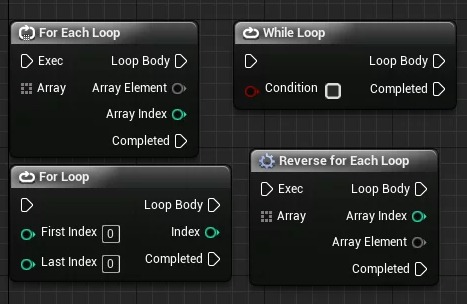
\includegraphics[height=5cm, width=13cm]{loop_blueprints.jpeg}
    \caption{Узлы для циклов}
\end{figure}
\begin{figure}[H]
    \centering
    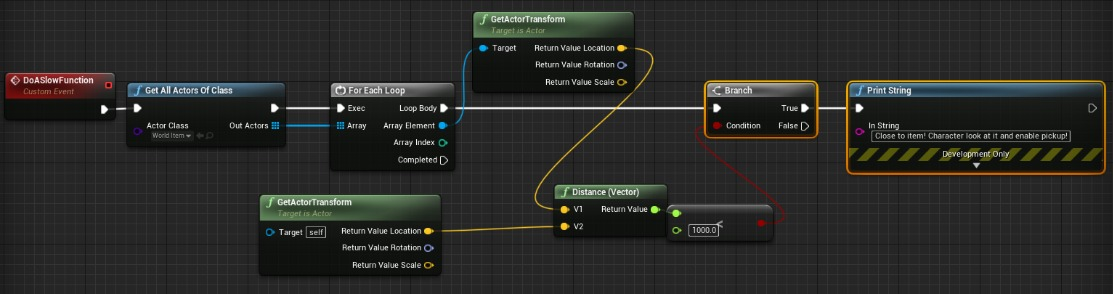
\includegraphics[height=7cm, width=13cm]{loop_example.jpeg}
    \caption{Пример итерирования по акторам с помощью for loop}
\end{figure}

\href{https://drive.google.com/file/d/1bpvySAOp3d32BuroTV2EeSUZdUUCpDe9/view?usp=drive_link}{\underline{Видео-демо по добавлению спринта для персонажа с помощью Blueprints}}

\subsection{Мультиребра в Unreal Engine 5}

В Unreal Engine 5 нет нативной поддержки мультиребер (multi-edges). Однако, похожий эффект можно достичь с помощью интерфейсов. Интерфейсы позволяют моделировать сложные связи между объектами и сущностями в игре, создавая гибкие и эффективные решения для взаимодействия между различными элементами сцены.

\href{https://dev.epicgames.com/documentation/en-us/unreal-engine/blueprint-interface-in-unreal-engine?application_version=5.1}{\underline{Документация по интерфейсам}}

\subsection{Взаимодействие C++ с Blueprints}

C++ и Blueprints могут работать вместе, что позволяет разработчикам создавать мощные и гибкие системы, сочетая производительность и низкоуровневое управление C++ с удобством и быстротой разработки Blueprints. Unreal Engine предоставляет множество способов интеграции C++ с Blueprints.
\newline
Одним из основных способов интеграции C++ и Blueprints является создание C++ классов и структур, которые можно использовать в Blueprints. Для этого необходимо создать новый класс, наследующийся от одного из базовых классов Unreal Engine, таких как \texttt{AActor}, \texttt{UObject}, или \texttt{UComponent}. При этом важно убедиться, что класс доступен для использования в Blueprints.

\begin{figure}[H]
    \centering
    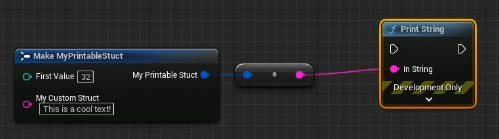
\includegraphics[height=4cm, width=10cm]{blueprints_with_cpp.jpeg}
    \caption{Взаимодействие написанной на C++ структры и Blueprint ноды print string}
\end{figure}

\subsection{Модели и Blueprints в Unreal Engine 5}

\subsubsection{Форматы моделей в Unreal Engine 5}

Unreal Engine 5 поддерживает несколько форматов для импорта и экспорта 3D моделей. Наиболее часто используемые форматы включают:

\begin{itemize}
    \item \textbf{FBX} (.fbx) — Один из наиболее популярных форматов для импорта моделей, анимаций и материалов в Unreal Engine. Он поддерживает сложные анимации, скелетные меши и данные о материалах, а также анимацию камеры и другие данные.
    \item \textbf{OBJ} (.obj) — Формат, часто используемый для импорта статичных 3D объектов. Он не поддерживает анимации и скелетные структуры, но подходит для простых моделей.
    \item \textbf{GLTF} (.glb, .gltf) — Формат для обмена 3D-моделями, который может содержать геометрию, материалы и анимации. Этот формат используется для передачи моделей в веб-приложениях и поддерживается многими современными движками и редакторами.
    \item \textbf{USD} (.usd, .usda, .usdc) — Формат для сцены и анимаций, поддерживающий сложные структуры сцен, шейдеры, материалы, а также анимацию.
\end{itemize}

Эти форматы совместимы с рядом популярных 3D редакторов, таких как \textbf{Blender}, \textbf{Maya}, \textbf{3ds Max} и других. Unreal Engine 5 также поддерживает прямой импорт из большинства этих программ, что упрощает процесс работы с 3D контентом.

\subsubsection{Где хранятся Blueprints в Unreal Engine 5}

Blueprints можно найти в структуре проекта Unreal Engine в каталоге \textbf{Content}, где они хранятся в виде активов, организованных в папки. Все активы, включая Blueprint'ы, находятся в каталоге \textit{Content}, а их формат — \textbf{.uasset}.

\subsection{Blueprints vs. C++}
Одна и та же функциональность написанная на Blueprints и C++
\begin{figure}[H]  % Use 'H' to force the figure to stay here
    \centering
    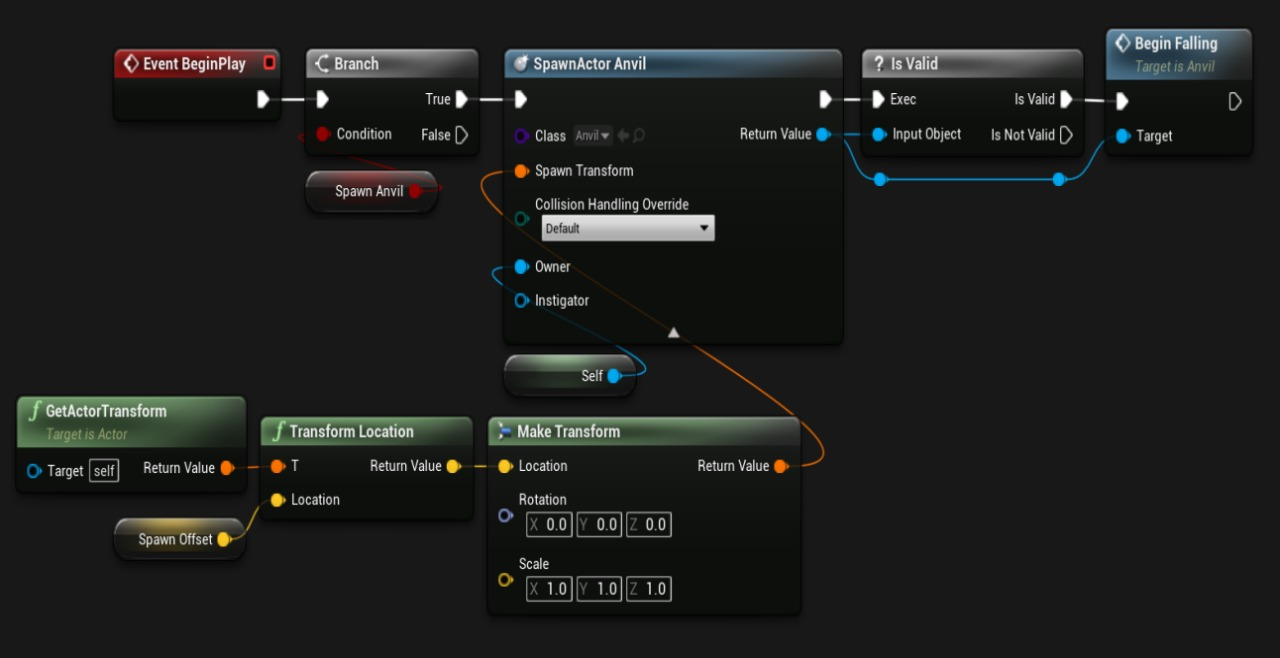
\includegraphics[height=8cm, width=13cm]{blueprints.jpeg}
    \caption{Blueprints.}

    \vspace{0.5cm} % Optional: Add vertical space between the two images

    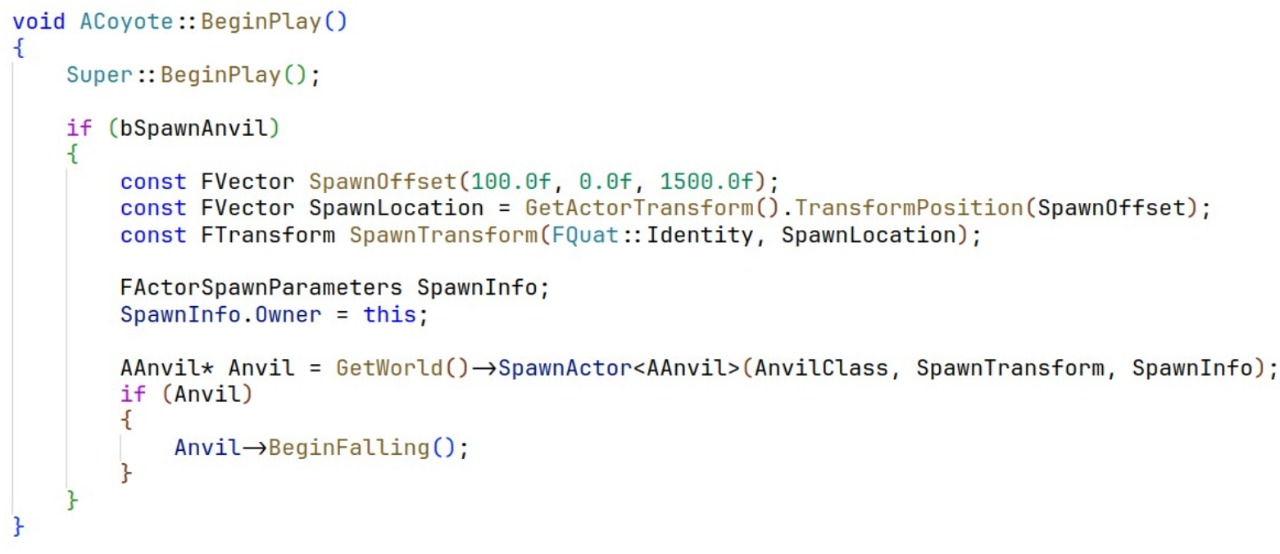
\includegraphics[height=7cm, width=13cm]{cpp.jpeg}
    \caption{C++.}
\end{figure}

\subsection{Процесс компиляции Blueprint}

Логика, написанная на Blueprints, компилируется в более низкоуровневое промежуточное представление, исполняемое на виртуальной машине, которое в конечном итоге сводится к исполнению скомпилированных C++ функций.

\begin{figure}[H]
    \centering
    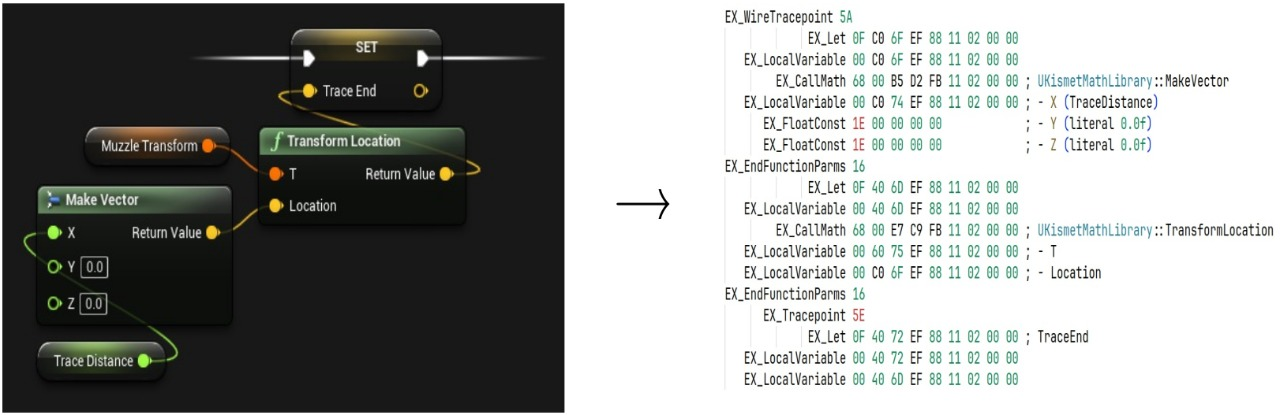
\includegraphics[height=7cm, width=13cm]{blueprints_ir.jpeg}
    \caption{Трансляция Blueprints в Промежуточное представление.}
\end{figure}

\subsection{Unreal Editor: Анимации}

Unreal Editor предлагает мощные инструменты для работы с анимациями, включая \textbf{AnimGraph} и \textbf{Blueprints}. Эти системы позволяют создавать, управлять и интегрировать анимации в проекты на платформе Unreal Engine.

\subsubsection{AnimGraph и Animations Blueprint}
\textbf{AnimGraph} — это визуальная система, предназначенная для создания сложных анимаций через соединение различных узлов и состояний. В связке с \textbf{Blueprints}, AnimGraph позволяет создавать динамичные анимационные схемы, где можно легко контролировать изменения состояния персонажей, объектов или камер в реальном времени. Animations Blueprint обеспечивают гибкость, позволяя создавать интерактивные анимации для игровых персонажей и объектов.

\subsubsection{Level Sequence Actor}
\textbf{Level Sequence Actor} Актор, который используется для создания и редактирования кинематографических последовательностей в Unreal Engine. Этот инструмент позволяет настраивать и управлять анимациями в контексте уровней и сцен, синхронизируя различные анимации.

\subsubsection{Ключевые кадры (Keyframes)}
Система \textbf{ключевых кадров} позволяет точно контролировать анимацию объекта или персонажа, записывая изменения их состояния на определённые моменты времени. Ключевые кадры в Unreal Engine являются основой для создания плавных переходов и динамичных изменений, обеспечивая большую гибкость при анимации движений, поз и других параметров в игре или кино.

Эти инструменты дают разработчикам огромные возможности для создания сложных, интерактивных анимаций, которые могут быть настроены для разных сценариев, что делает процесс анимации более эффективным и гибким.

\href{https://drive.google.com/file/d/1hCq_oF2frF_jmGwil24nNf5JegSw5t2a/view?usp=drive_link}{\underline{Видео-демо по созданию анимации с нуля}}
\newline
\href{https://drive.google.com/file/d/1bpvySAOp3d32BuroTV2EeSUZdUUCpDe9/view?usp=drive_link}{\underline{Видео-демо по добавлению созданной анимации к персонажу}}

\subsection{Заключение. Почему стоит выбрать Unreal Engine?}

\subsubsection{Open-source}
Unreal Engine является \textbf{open-source} (с открытым исходным кодом), что дает разработчикам полный доступ ко всем его компонентам. Это позволяет не только модифицировать и адаптировать движок под специфические нужды проекта.

\subsubsection{Стандарт индустрии}
Unreal Engine уже давно зарекомендовал себя как \textbf{стандарт индустрии} в области разработки игр и интерактивных приложений. Множество крупных студий и проектов выбирают Unreal благодаря его высокой производительности и продвинутым инструментам.

\subsubsection{Производительность}
Одним из главных преимуществ Unreal Engine является его исключительная \textbf{производительность}. Движок оптимизирован для работы с высококачественной графикой, и его возможности позволяют эффективно использовать ресурсы системы для обеспечения максимальной производительности как на консолях, так и на ПК.

\subsubsection{Поддержка и сообщество}
\textbf{Поддержка} и активное \textbf{сообщество} разработчиков — это ещё один важный аспект, который делает Unreal Engine отличным выбором. Epic Games активно поддерживает пользователей своего движка, регулярно выпуская обновления, исправления и улучшения.

\subsubsection{Обилие учебных материалов}
Для начинающих и опытных разработчиков доступно огромное количество \textbf{учебных материалов}. В интернете можно найти официальные документации, курсы, видеоуроки и форумы, где люди делятся опытом и отвечают на вопросы. Epic Games также предоставляет доступ к множеству бесплатных ресурсов, включая учебные проекты, шаблоны и примеры кода. Это значительно ускоряет процесс обучения и помогает разработчикам быстро освоить возможности Unreal Engine.

}

\newcommand{\lecture}[2]{
    \section{#1}
    \begin{center}
        Конспект составил(а): \textit{#2}
    \end{center}
}

\newcommand{\report}[2]{
    \section{Отчет по докладу \foreignquote{russian}{#1}}
    \begin{center}
        Отчет составил(а): \textit{#2}
    \end{center}
}
